% ---------------------------------------------------------------------
% --- Arquivo principal e os demais serao os dos capitulos.
% --- EXPRESSÔES ENTRE <> DEVERÂO SER COMPLETADAS COM A INFORMAÇÂO ESPECÌFICA DO TRABALHO 
% ---------------------------------------------------------------------
\documentclass[ruledheader]{abnt_UFF}[abntex2]
\usepackage[alf]{abntex2cite}

%--- pacotes para hiphenizacao e acentuacao em portugues
\usepackage[brazil]{babel}
%\usepackage[latin1]{inputenc}
\usepackage[utf8]{inputenc}
\usepackage[T1]{fontenc}

%--- pacote para figuras
\usepackage{epsf}
\usepackage[dvips]{epsfig,graphicx}
\usepackage{subfigure}

%--- pacote de simbolos
\usepackage{latexsym}
\usepackage{textcomp}

%--- simbolos matematicos
\usepackage{amsmath}
\usepackage{amssymb}

%--- pacote para gerar pseudo-codigo
\usepackage{algorithm}
\usepackage{algorithmic}
\floatname{algorithm}{Algoritmo}

%--- outros pacotes
\usepackage{url}
\usepackage{longtable}
\usepackage{pdflscape}
\usepackage{setspace}
\usepackage{booktabs}
\usepackage{alltt}
\usepackage[flushleft]{threeparttable}
\renewcommand{\ttdefault}{txtt}

%Tabela Colorida
\usepackage{colortbl}
\usepackage{multicol}
\usepackage{multirow}
\usepackage{rotating}

\hyphenation{
    a-de-qua-da-men-te
    di-men-sio-na-men-to
}

%---------usando tipo de fonte padrao
\renewcommand{\ABNTchapterfont}{\bfseries\fontfamily{cmr}\fontseries{b}\selectfont}
\renewcommand{\ABNTsectionfont}{\bfseries\fontfamily{cmr}}

% --- -----------------------------------------------------------------
% --- Documento Principal.
% --- -----------------------------------------------------------------
% \usepackage[pdftex]{hyperref}
% \hypersetup{colorlinks, sitecolor=black, pdftex}

\begin{document}
    % --- Para elementos em português, remover.
    \renewcommand{\listfigurename}{Lista de Figuras}
    \renewcommand{\figurename}{Figura}
    \renewcommand{\listtablename}{Lista de Tabelas}
    \renewcommand{\tablename}{Tabela}
    \renewcommand{\contentsname}{Sumário}
    \renewcommand{\refname}{Referências}
    \renewcommand{\appendixname}{Apêndices}
    \renewcommand{\chaptername}{Capítulo}

% --- -----------------------------------------------------------------
% --- Titulo, abstract, dedicatorias e agradecimentos.
% --- Indice geral, lista de figuras e tabelas.
% --- -----------------------------------------------------------------
    	% --- -----------------------------------------------------------------
	% --- Elementos usados na Capa e na Folha de Rosto.
	% --- EXPRESS�ES ENTRE <> DEVER�O SER COMPLETADAS COM A INFORMA��O ESPEC�FICA DO TRABALHO
	% --- E OS S�MBOLOS <> DEVEM SER RETIRADOS 
	% --- -----------------------------------------------------------------
	\cleardoublepage
	\thispagestyle{empty}
	
	\vspace{-60mm}
	  \begin{singlespace}
	    \begin{center}
	      {\large UNIVERSIDADE FEDERAL DO ACRE}
	      \vskip4.0cm{\textbf{\Large Gustavo Moreira Oliveira de Castro}}
	      \vskip5.0cm {\textbf{Estimação de mapas de profundidade em imagens de câmeras monoculares utilizando modelos de difusão}}
	    \end{center}
	    \begin{center}
	      \vskip10.0cm{\textbf{RIO BRANCO\\2024}}
	    \end{center}
	  \end{singlespace}
	% --- -----------------------------------------------------------------
	% --- Folha de rosto. (Obrigatorio)
	% --- ----------------------------------------------------------------
	\cleardoublepage
	\thispagestyle{empty}
	
	\vspace{-60mm}
	  \begin{center}
	    {\large UNIVERSIDADE FEDERAL DO ACRE}\\
	    \vspace{3cm}
	    {\large Gustavo Moreira Oliveira de Castro} \\
	    \vspace{3cm}
	    
	    {\large Estimação de mapas de profundidade em imagens de câmeras monoculares utilizando modelos de difusão} \\
	    \vspace{1.5cm}
	  \end{center}
	
	\noindent
	  \begin{flushright}
	    \begin{minipage}[t]{8cm}
	     \textcolor{red}{Proposta de dissertação de mestrado submetida ao Programa de Pós-Graduação em Ciência da Computação na Universidade Federal do Acre como requisito parcial para obtenção do título de mestre em Ciência da Computação. Linha de Pesquisa: Sistemas Computacionais Inteligentes}
	    \end{minipage}
	  \end{flushright}
	
	\vskip1.50cm
	  \begin{center}
	    \small Orientadora: \\
	    Prof. Dr. {Roger Fredy Larico Chavez}\vskip3.5cm 
	  \end{center}
	  \begin{center}
	    \vspace{4mm}
	    RIO BRANCO \\
	    %\vspace{6mm}
	    2024
	  \end{center}
	
	\thispagestyle{empty}
	% --- -----------------------------------------------------------------
	% --- Termo de aprovacao. (Obrigatorio)
	% --- ----------------------------------------------------------------
	\cleardoublepage
	\thispagestyle{empty}
	
	\vspace{-60mm}
	
	\begin{center}
	  {\large Gustavo Moreira Oliveira de Castro} \\
	  \vspace{7mm}
	
	  {\large Estimação de mapas de profundidade em imagens de câmeras monoculares utilizando modelos de difusão} \\
	  \vspace{10mm}
	\end{center}
	
	\noindent
	\begin{flushright}
	  \begin{minipage}[t]{8cm}
	
		\textcolor{red}{Proposta de dissertação de mestrado submetida ao Programa de Pós-Graduação em Ciência da Computação na Universidade Federal do Acre como requisito parcial para obtenção do título de mestre em Ciência da Computação. Linha de Pesquisa: Sistemas Computacionais Inteligentes}.
	
	  \end{minipage}
	\end{flushright}
	
	\vspace{1.0 cm}
	\noindent
	
	Approved in <MONTH> of <YEAR>. \\
	\begin{flushright}
	  \parbox{11cm}
	  {
	    \begin{center}
	      \vspace{3mm}
	      \rule{11cm}{.1mm} \\
	      Prof. Dr. Roger Fredy Larico Chavez\\
	      Universidade Federal do Acre
	      \vspace{3mm}
	    \end{center}
     
     \begin{center}
	      \vspace{3mm}
	      \rule{11cm}{.1mm} \\
	      Prof. Dr. ...\\
	      Universidade Federal do Acre
	      \vspace{3mm}
	    \end{center}
     
     \begin{center}
	      \vspace{3mm}
	      \rule{11cm}{.1mm} \\
	      Prof. Dr. ...\\
	      Universidade Federal do Acre
	      \vspace{3mm}
	    \end{center}
	  }
	\end{flushright}
	
	\begin{center}
	  \vspace{4mm}
	  RIO BRANCO \\
	  %\vspace{6mm}
	  2024
	\end{center}
	
	% --- -----------------------------------------------------------------
	% --- Dedicatoria.(Opcional)
	% --- ----------------------------------------------------------------
	\cleardoublepage
	\thispagestyle{empty}
	\vspace*{200mm}
	
	\begin{flushright}
	  {\em
	dfsaas
	    \\
	   - 
	    \\ 
	    
	  }
	\end{flushright}
	\newpage
	
	% --- -----------------------------------------------------------------
	% --- Agradecimentos.(Opcional)
	% --- ----------------------------------------------------------------
	\pretextualchapter{Agradecimentos}
	\hspace{5mm}
	
	...
	
	% --- -----------------------------------------------------------------
	% --- Resumo em portugues.(Obrigatorio)
	% --- ----------------------------------------------------------------
	\begin{resumo}
	
	  \begin{center}{
	    \textbf{Estimação de mapas de profundidade em imagens de câmeras monoculares utilizando modelos de difusão}}
	  \end{center}
	
	\begin{spacing}{1.0}
	  ...
	\end{spacing}
	{\hspace{-8mm} \bf{Palavras-chave}}: ...; ...; ...; ....
	
	\end{resumo}
	
	% --- -----------------------------------------------------------------
	% --- Resumo em lingua estrangeira.(Obrigatorio)
	% --- ----------------------------------------------------------------
	\begin{abstract}
	
	....
	
	{\hspace{-8mm} \bf{Keywords}}: Regression; GAMLSS; OLLST; Repeated measure in time
	
	\end{abstract}
	
	% --- -----------------------------------------------------------------
	% --- Lista de figuras.(Opcional)
	% --- -----------------------------------------------------------------
	%\cleardoublepage
	\listoffigures
	
	% --- -----------------------------------------------------------------
	% --- Lista de tabelas.(Opcional)
	% --- -----------------------------------------------------------------
	\cleardoublepage
	%\label{pag:last_page_introduction}
	\listoftables
	\cleardoublepage
	
	% --- -----------------------------------------------------------------
	% --- Sumario.(Obrigatorio)
	% --- -----------------------------------------------------------------
	\pagestyle{ruledheader}
	\tableofcontents
	
% --- -----------------------------------------------------------------
% --- Insercao dos capitulos.
% --- -----------------------------------------------------------------
    \pagestyle{ruledheader}
    \setcounter{page}{1}
    \pagenumbering{arabic}
    
\chapter{Introdução}

Informação de profundidade é uma das representações mais úteis para o entendimento de ambientes físicos \cite{lasinger2019towards} \cite{zhou2019does}. São também uma parte importante da caracterização de relações geométricas de uma determinada cena. As imagens de profundidades (ou mapas de profundidade) desempenham um papel importante em uma série de aplicações que envolvem visão computacional \cite{eigen2014depth}.  Entre elas, podemos citar: compreensão de cenas \cite{jaritz2018sparse}, veículos autônomos \cite{song2021self}, navegação de robôs \cite{ma2019sparse} navegação de VANTs, \cite{padhy2023monocular} fazendas inteligentes \cite{farkhani2019sparse}, e realidade aumentada \cite{du2020depthlab}. 

% \textit{Simultaneos Localization and Mapping} (SLAM) \cite{hu2012robust}

Os mapas de profundidade representam as distâncias de cada ponto (ou pixel) numa cena física em relação ao eixo do dispositivo de captura. Podem ser representados por imagens em escala de cinza, com as cores dos pixels sendo proporcionais à distância, com cinzas mais claros para objetos mais próximos e tons mais escuros para pontos mais afastados (e vice-versa), como exemplificado na Figura \ref{dmap}, que mostra uma cena em imagem RGB, seu mapa de profundidade e uma versão colorizada. Pontos cuja medição é desconhecida são representados por pixels totalmente pretos ou totalmente brancos \cite{dourado2020multi}.

\begin{figure}[h]
    \centering
    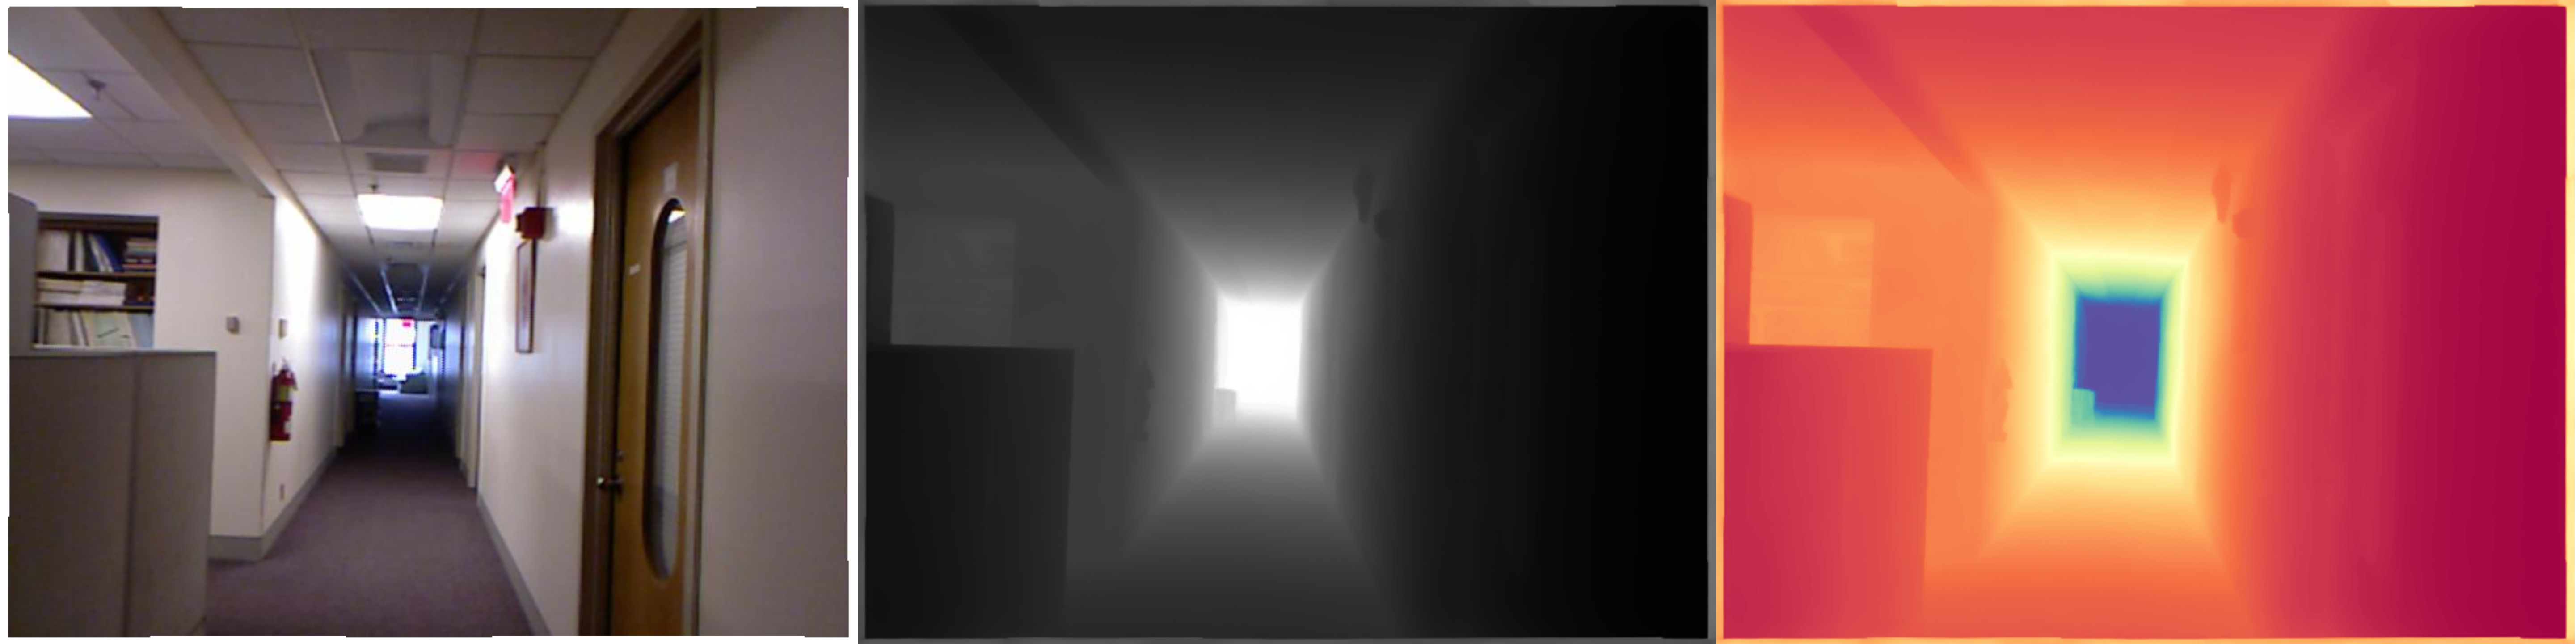
\includegraphics[width=\textwidth]{fig/example_depth.png}
    \caption{Exemplo de mapa de profundidade do \textit{dataset Nyu Depth V2}. No primeiro quadro, a imagem RGB, no segundo, o mapa de profundidade em escala de cinza, no terceiro uma colorização artificial para o mapa de profundidade.}
    \label{dmap}
\end{figure}


Para capturar tais imagens geralmente são empregadas câmeras RGB-D, que podem prover tanto informação de profundidade quanto imagens coloridas da cena. Entre suas tecnologias mais comuns, são encontrados diversos tipos de aquisição que podem ser baseados em visão estereoscópica, que trabalha com múltiplos ângulos de visão, sensores \textit{Time-of-Flight} (ToF) que emprega projeção de lasers infravermelhos (IR) estruturados e técnicas mais precisas como o LiDAR (\textit{Light Detection and Ranging}) \cite{castellano2023performance}.


Sensores de profundidade estão cada vez mais embarcados em equipamentos amplamente difundidos como dispositivos de realidade aumentada (Occulus, Kinnect) e até mesmo em smartphones \cite{du2020depthlab}, principalmente as câmeras ToF, pois são capazes de desempenhar de maneira satisfatória mesmo com baixa potência \cite{branscombe2018microsoft}. De acordo com \cite{xie2021ultradepth}, a adoção de sensores de profundidade em smartphones tende a aumentar nos próximos anos, com diversas aplicações como tradução de linguagem de sinais \cite{park2021enabling} e sistemas de navegação mobile para pessoas com deficiência visual \cite{see2022smartphone}.

%sinal 57, gestos 86, e aumentada 97

Ainda segundo \cite{castellano2023performance}, cada uma das técnicas de aquisição de imagens de profundidade possui lados negativos que podem impactar os dados. Por exemplo, as câmeras ToF podem sofrer com invalidação de pixels próximo a cantos ou bordas de objetos devido à interferências entre os raios IR em superfícies descontínuas ou reflexivas \cite{hansard2012time}, exemplificado na Figura \ref{errdepth}. Outros tipos de câmeras RGB-D mais comuns como o Microsoft Kinect ou Intel RealSense podem produzir valores inválidos em superfícies muito brilhantes ou reflexivas como espelhos, superfícies metálicas ou muito escuras \cite{zollhofer2019commodity}. Em ambientes internos, tais imagens podem conter até 50\% de dados faltantes. \cite{zhang2022indepth} \cite{zhang2018deep}. 

\begin{figure}
    \centering   
    \includegraphics[width=\textwidth]{fig/depth_problema.png}
    \caption{Exemplo de imagem RGB com mapa de profundidade apresentando leituras inválidas.}
    \label{errdepth}
\end{figure}

%problemas 27, 80, 98

Garantir a correta representação dos mapas em escala de pixel é de considerável importância para as tarefas que dependem de profundidade e que requerem um alto grau de segurança e confiabilidade dos dados, como veículos autônomos ou navegação de drones. A tecnologia LiDAR é a alternativa com implementação mais confiável entre as que foram citadas, no entanto, ressalta-se que nem o LiDAR e nem câmeras RGB-D convencionais produzem mapas completos e densos \cite{hu2012robust}. 

Ainda de acordo com \cite{hu2012robust}, o problema de preenchimento de valores indeterminados em mapas de profundidade depende inteiramente do sensor utilizado para sua captura. No caso do LiDAR, são produzidos mapas esparsos (approx. 95\% de esparsidade) e no caso de câmeras RGB-D ou câmeras ToF são produzidos mapas com partes faltantes em determinadas superfícies ou bordas. Os pixels inválidos normalmente são representados pelo valor 0 \cite{dourado2020multi}. De acordo com \cite{zhang2018deep}, o problema de correção de imagens de profundidade implica em fazer novas predições para áreas em que o sensor não retornou dados válidos.

Neste cenário, o presente trabalho apresenta uma abordagem baseada em técnicas de \textit{inpainting} utilizando redes neurais artificiais para realizar a correção de erros de mapas de profundidade capturados por câmeras RGB-D e sensores ToF.



% Neste cenário, tecnologias de aquisição e melhoramento dos dados foram amplamente pesquisadas pela ciência nos últimos anos. Recentemente foram exploradas técnicas que não dependem de sensores de profundidade, ou seja, que inferem a informação de profundidade a partir de uma única imagem RGB capturada a partir de uma câmera comum, essa abordagem é conhecida como \textit{Monocular Depth Estimation} (MDE). No entanto, métodos baseados em características puramente visuais   \cite{szeliski2022computer} \cite{hu2022deep}. 

     
	    
\subsection{Trabalhos Relacionados}          


\section{Motivação} 

		

 
\section{Objetivos}


\subsection{Objetivo Geral}
Este trabalho possui como objetivo geral realizar a correção de mapas de profundidade com erros através de redes neurais artificiais e técnicas de \textit{inpainting}.

\subsection{Objetivos Específicos}

\begin{itemize}
    \item Realizar revisão de literatura de métodos de correção de mapas de profundidade.
    \item Escolher um método de \textit{inpainting} baseado em redes neurais artificiais.
    \item Estabelecer um método de geração de máscaras de erro para treinamento.
    \item Corrigir mapas de profundidade com algoritmo de \textit{inpainting} baseado em correção não-guiada.
    \item Corrigir mapas de profundidade com algoritmo de \textit{inpainting} baseado em correção guiada.
    \item Corrigir mapas de profundidade utilizando abordagem morfológica.
    \item Comparar as diferentes abordagens através de métricas de avaliação perante a diferentes níveis de pixels inválidos.
    
\end{itemize}

\chapter{Revisão Bibliográfica}


\chapter{Marco Teórico}

\section{}



\chapter{Materiais e Métodos}

\subsection{Correção de mapas de profundidade} 

Para a tarefa de correção de mapas de profundidade utilizando redes neurais, o trabalho de \cite{hu2022deep} propôs duas categorias principais que se diferenciam pelos dados utilizados:

\begin{itemize}
    \item \textbf{Correção não-guiada} (Figura \ref{ung}): Objetiva completar diretamente as partes faltantes utilizando como entrada somente o mapa de profundidade.
    \item \textbf{Correção guiada} (Figura \ref{early} e \ref{late}): Objetiva completar as partes faltantes utilizando como entrada tanto o mapa de profundidade quanto a imagem RGB correspondente.
\end{itemize}

\begin{figure}[h]
    \centering
    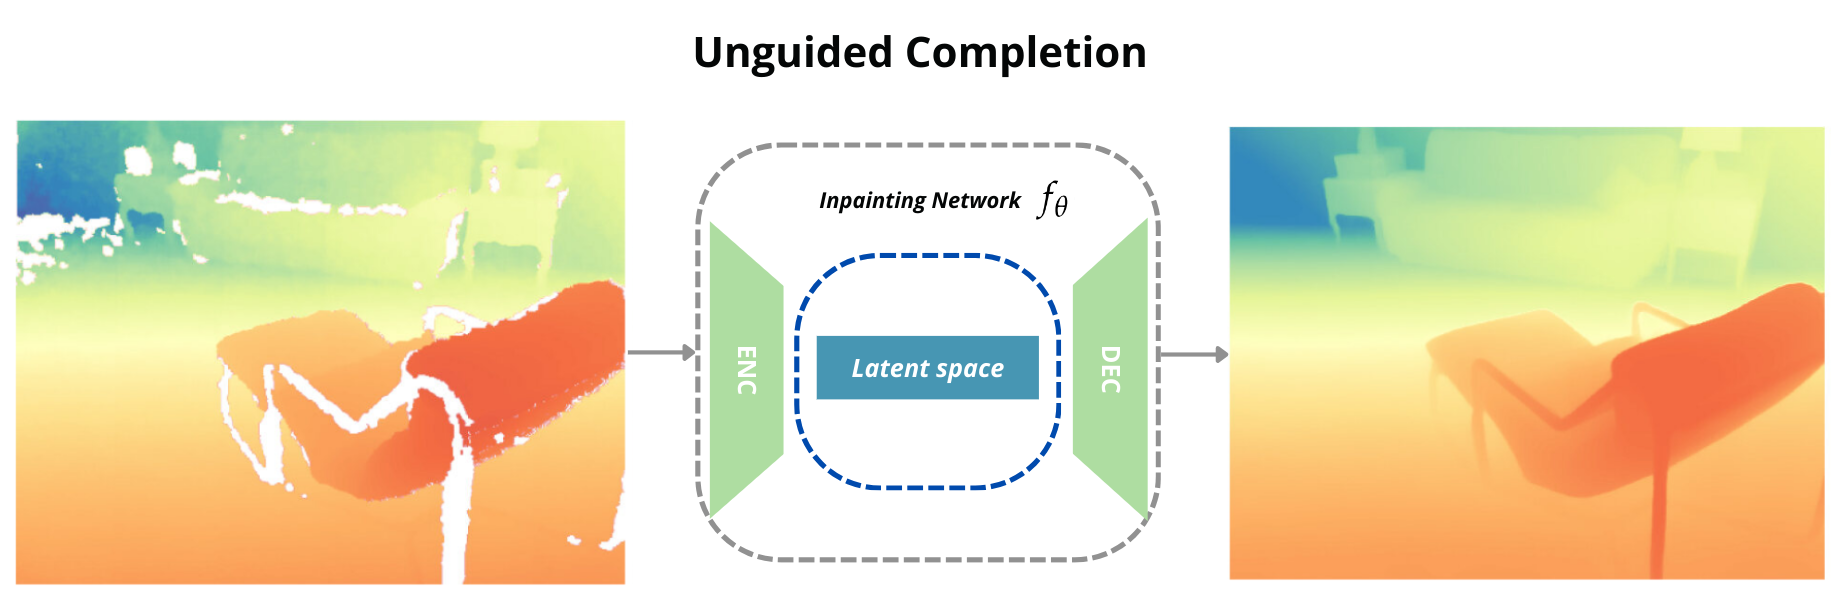
\includegraphics[width=\textwidth]{fig/unguided.png}
    \caption{Esquema de correção não-guiada.}
    \label{ung}
\end{figure}

A escolha da categoria de correção depende da quantidade de erros nas imagens. Quando há uma pequena quantidade de pixels inválidos, a correção não-guiada pode ser adequada, visto que não é necessário uma profunda extração de características dos dados. No entanto, no caso contrário, o uso de métodos guiados é indicado dado que existam grandes regiões com ausência de informação de profundidade ou que o mapa apresente uma grande esparsidade. Sendo necessário recorrer a extração dos atributos presentes na imagem RGB como bordas, contornos, estruturas de objetos não identificados pelo sensor e característica de descontinuidade de superfícies \cite{hu2022deep}.

Ainda no trabalho de \cite{hu2022deep}, nomeia-se outras subcategorias de técnicas de correção guiada. Uma delas é chamada de \textit{Early Fusion} (Figura \ref{early}) e consiste em utilizar a imagem RGB concatenada ao mapa de profundidade com erros como entrada da rede neural. Essa técnica possui a vantagem de ser simples e de baixa complexidade. A outra, conhecida como \textit{Late Fusion} (Figura \ref{late}) envolve transferir a fusão da imagem RGB com o mapa em ramos distintos da rede neural, chamados \textit{RGB Encoder-Decoder} e \textit{Depth Encoder-Decoder}.

\begin{figure}[h]
    \centering
    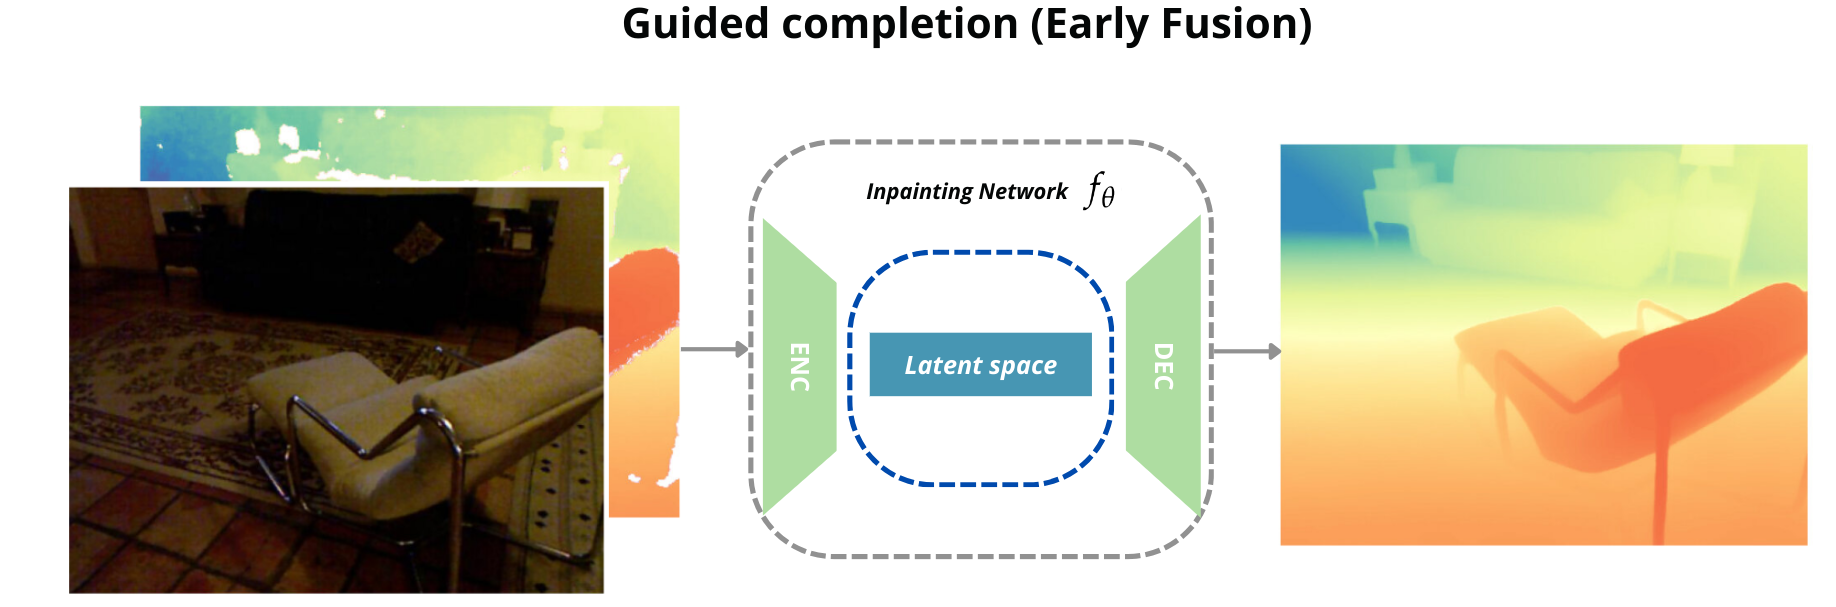
\includegraphics[width=\textwidth]{fig/earlyfusion.png}
    \caption{Esquema de correção guiada com \textit{Early Fusion}.}
    \label{early}
\end{figure}

\begin{figure}[h]
    \centering
    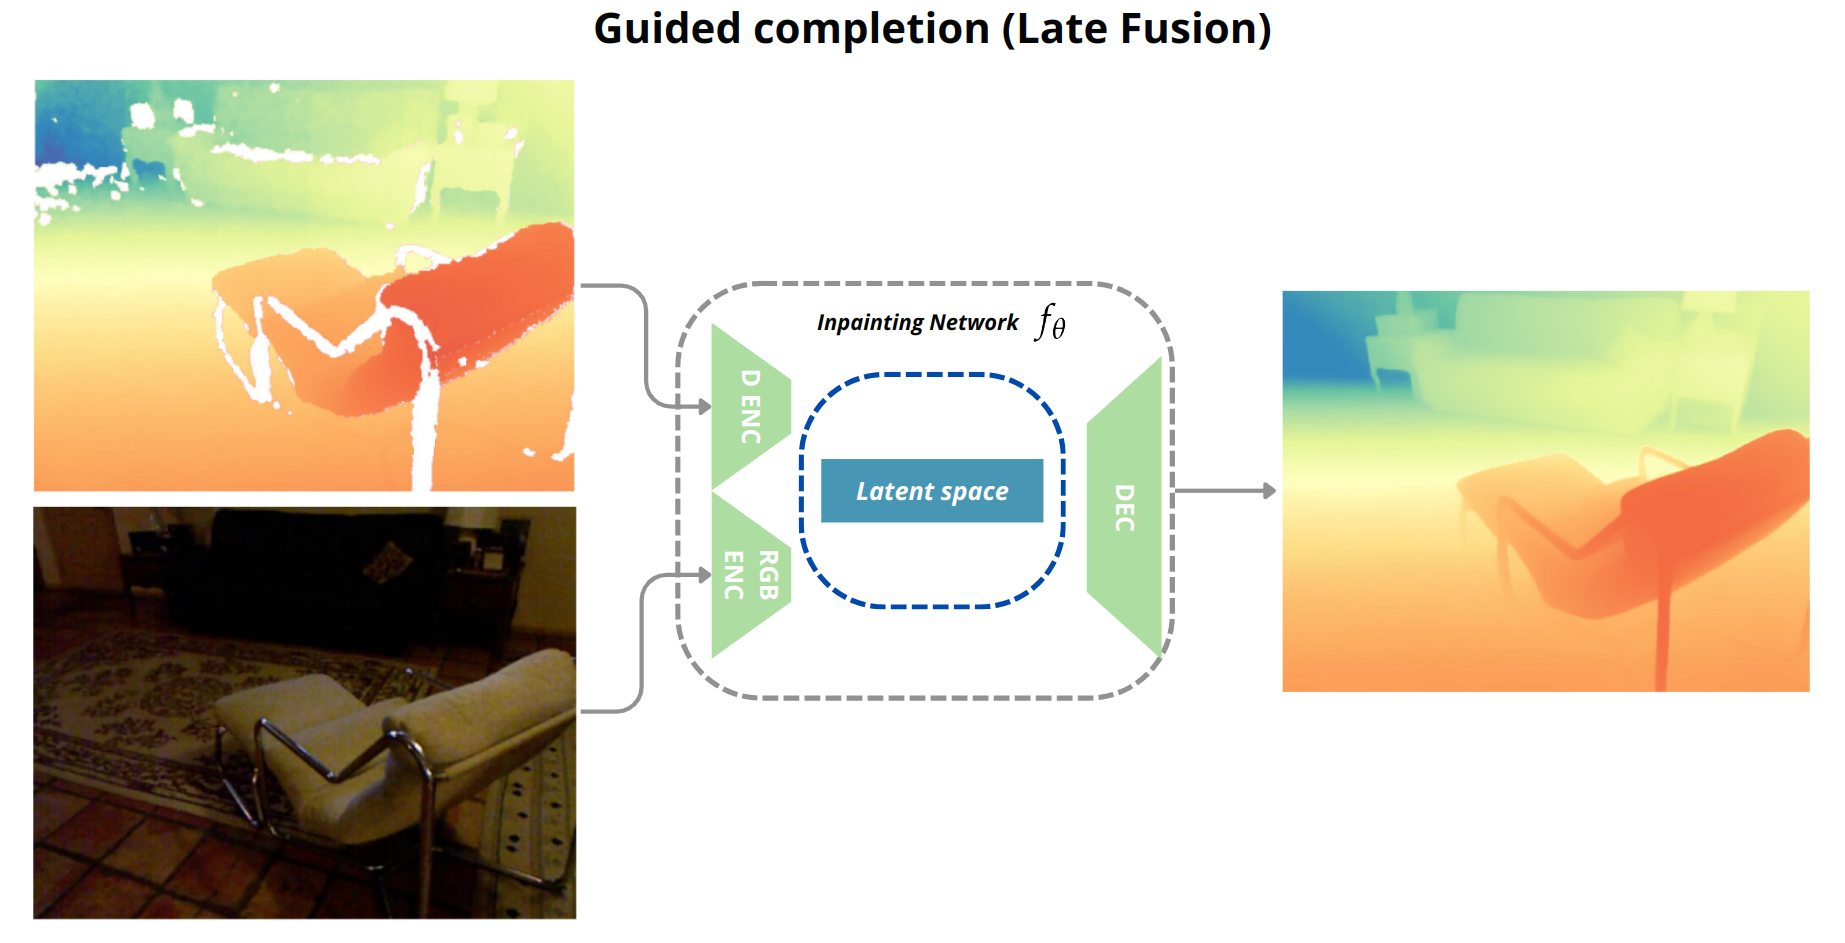
\includegraphics[width=\textwidth]{fig/latefusion.png}
    \caption{Esquema de correção guiada com \textit{Late Fusion}.}
    \label{late}
\end{figure}


\subsection{Large Mask Inpainting}

%Image inpainting is the process of completing or recovering the missing region in the image or removing some objects added to it. 

\textit{Image Inpainting} refere-se ao processo de recuperar regiões faltantes de uma imagem a partir de informação já existente \cite{elharrouss2020image}. Para sintetizar as partes indicadas, é necessário que haja o aprendizado da estrutura global da imagem, sendo imprescindível um vasto campo receptivo na rede neural. Dessa forma, é proposto por \cite{suvorov2022resolution} o sistema LaMa, \textit{Large Mask Inpainting} (Figura \ref{lama}), que é composto por elementos capazes de explorar o campo receptivo apropriado para essa tarefa, sendo eles: i) convoluções rápidas de Fourier (do inglês, \textit{Fast Fourier Convolutions}), ii) o uso de perda perceptual baseada em uma rede de segmentação e iii) uma estratégia de geração de máscaras para treinamento de alta cobertura.

\begin{figure}[h]
    \centering
    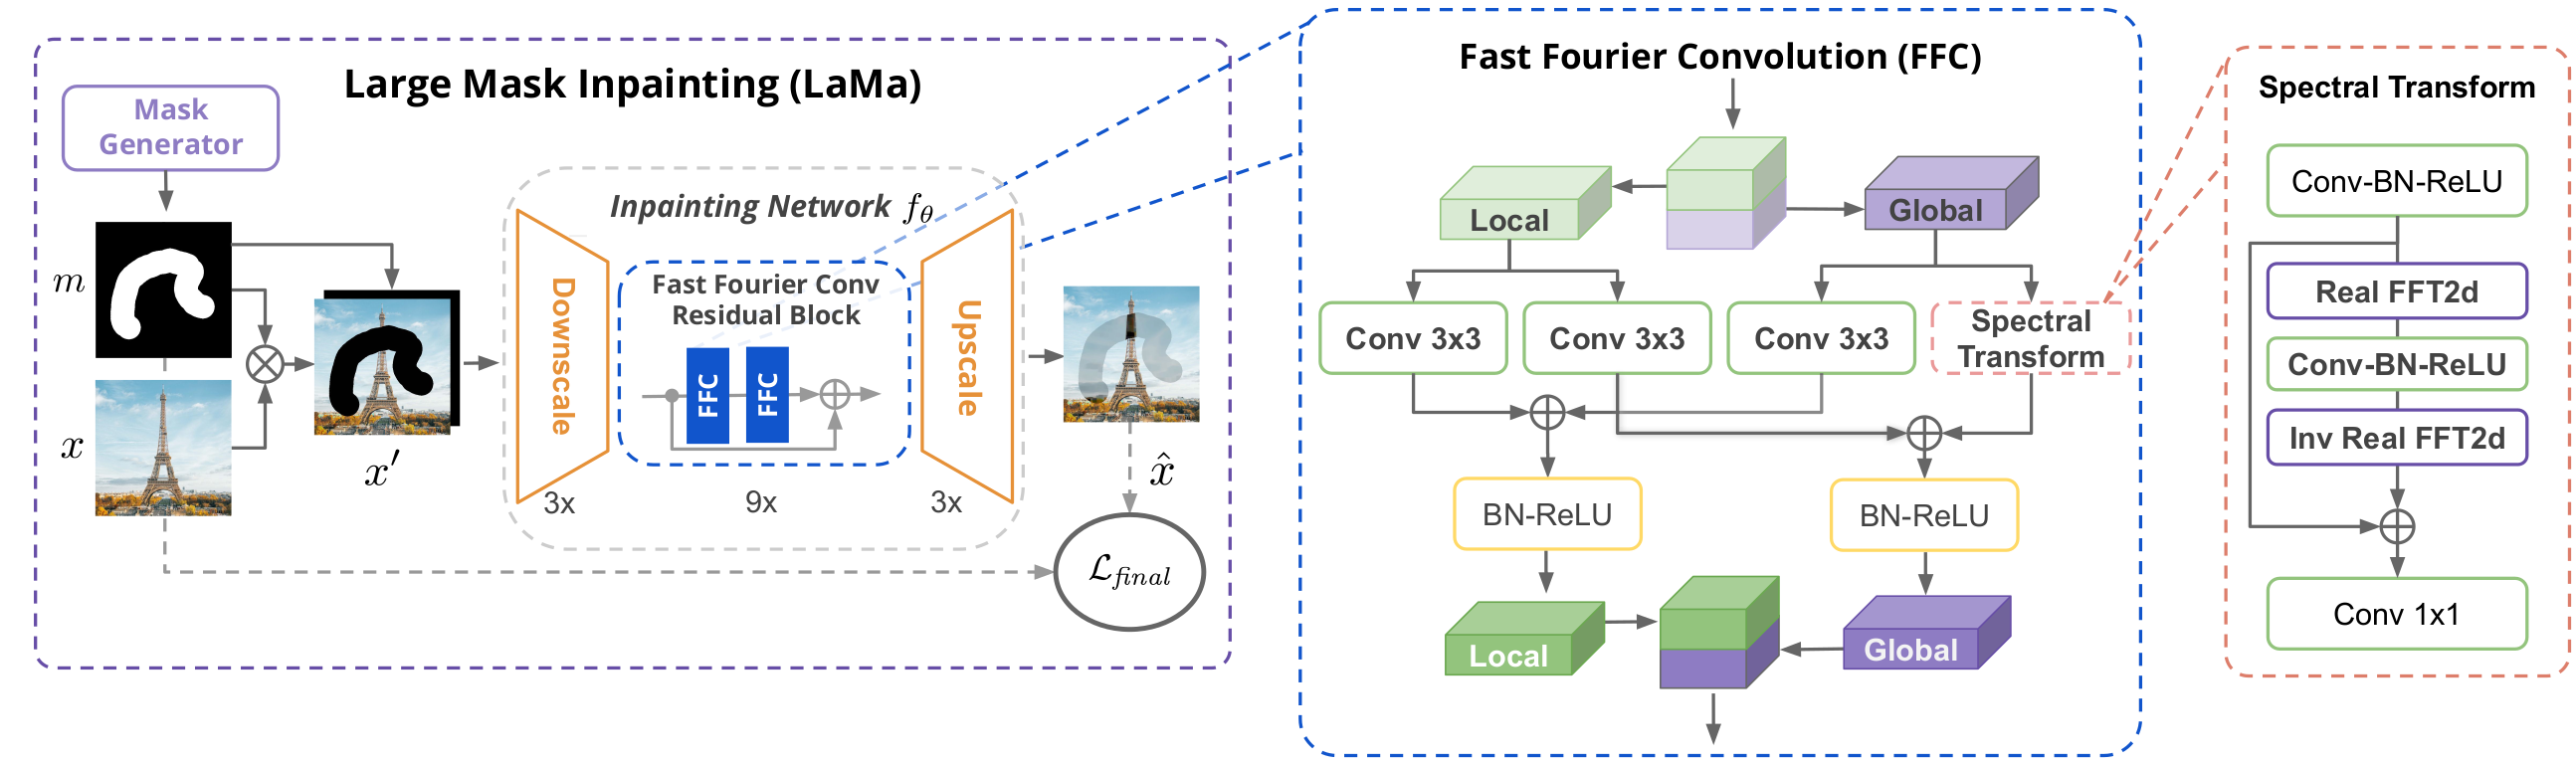
\includegraphics[width=\textwidth]{fig/lama.png}
    \caption{Esquema do método LaMa \cite{suvorov2022resolution}.}
    \label{lama}
\end{figure}

%explain receptive field?

\section{Datasets}

O presente trabalho exige um tipo de base de dados pouco encontrado na literatura, trios de imagem RGB, mapa de profundidade com erros e um outro mapa de profundidade denso e completo. De acordo com \cite{zhang2018deep}, uma das maneiras de se obter esses dados seria capturar imagens com uma câmera RGB-D de baixo custo e alinha-las com outra captura simultânea de um sensor mais preciso, porém essa abordagem é muito custosa, além de que não há disponibilidade de grandes conjuntos para treinamento.

O presente projeto pretende utilizar como base de dados principal o \textbf{Hypersim}. Um \textit{dataset} para compreensão de cenas baseado em cenas sintéticas fotorrealistas. Contendo 77.400 imagens de 461 cenas \textit{indoor} com pares de RGB e mapas de profundidade calculado deterministicamente, além de outras informações como normais de superfície, rótulos de segmentação e detecção de objetos e entre outros \cite{roberts2021hypersim}.

\section{Metodologia da Pesquisa}





\chapter{Resultados Preliminares}








    \chapter{Trabalhos Relacionados}

%COMMENT -----------------------------------------------------------
\textcolor{red}{acho que vale a pena organizar os trabalhos por método empregado, i) métodos determinísticos (não inteligentes), ii) redes neurais convolucionais, iii) transformers, iv) modelos generativos (gans e diffusion e lama e oq mais tiver)}

Em \citeonline{liu2012guided} foi proposto um algoritmo de \textit{inpainting} para aprimorar os mapas de profundidade capturados com Kinect, estendendo o método original de marcha rápida (\textit{Fast Marching Method} - FMM) para reconstruir regiões desconhecidas incorporando uma imagem RGB alinhada como guia. Em seguida, aplica-se um filtro de preservação de bordas para reduzir o ruído nas regiões de separação de objetos. 

No trabalho de \citeonline{zhang2018deep}, foi desenvolvido um esquema que utiliza uma rede neural para inferir as normais de superfície e os limites de oclusão a partir de uma imagem RGB. Essas predições são combinadas com mapas de profundidade de câmeras RGB-D através de um método de otimização para computar a profundidade resultante de todos os pixels da imagem. A rede neural possui arquitetura totalmente convolucional utilizando a VGG-16 como \textit{backbone} e é treinada com as normais de superfície e limites de oclusão computados a partir da renderização de uma malha tridimensional reconstruída a partir de múltiplos ângulos de visão. 
 

\citeonline{dourado2020multi} introduz o método NSGA2CGP, uma abordagem de otimização multi-objetivo que integra programação cartesiana genética para a otimização de filtros morfológicos em escala de cinza para completar mapas de profundidade utilizados para algoritmo detector de caminho livre. O objetivo é minimizar tanto os erros quanto a complexidade dos elementos estruturantes dado as limitações energéticas dos sistemas de navegação embarcados para pessoas com deficiência visual. Além do erro, também foram mensurados na aplicação, o consumo de energia e tempo de execução. 


É proposto por \citeonline{fujii2020rgb} um método para \textit{inpainting} de imagens RGB-D utilizando uma rede generativa adversarial (\textit{Generative Adversarial Network} - GAN) objetivando restaurar simultâneamente a textura e geometria de regiões faltantes levando em consideração as informações complementares de cor e profundidade com uma abordagem de fusão tardia, resultando na restauração tanto dos canais RGB quanto de mapas de profundidade.

Com o objetivo de complementar o trabalho de \citeonline{zhang2018deep}, os autores \citeonline{huang2019indoor} desenvolveram um \textit{framework} para completar mapas de profundidade buscando preservar a clareza das bordas dos objetos mantendo a estrutura da imagem, evitando o cenário onde as redes neurais aprendem meramente a interpolar os valores de profundidade. É empregado o mecanismo de atenção própria para reunir informação das características de normais de superfície e limites de oclusão. Os autores afirmam que são alcançados tempos de execução menores em relação ao estado da arte.


Em \citeonline{rho2022guideformer}, é apresentada uma arquitetura para correção de mapas de profundidade esparsos em três estágios. Uma estrutura dupla de \textit{encoder-decoder} baseada em \textit{transformers} para extrair características dos \textit{tokens} das imagens RGB e mapas de profundidade esparsos. Um módulo de atenção guiada (GAM, do inglês \textit{Guided-Attention Module}) para fusionar os dados das duas modalidades distintas. Um método para fusionar os resultados dos ramos e capturar as dependências intermodais. \textcolor{red}{talvez não tenha ficado bem explicado}


Ainda utilizando GANs, \citeonline{wang2022rgb} propôs uma rede de dois ramos projetada para estimar mapas de profundidade completos a partir de pares de mapas de profundidade incompletos e imagens RGB. No primeiro ramo, uma estrutura de \textit{encoder-decoder} é empregada para predizer valores de profundidade densos. No segundo ramo, é utilizada uma estrutura de GAN que possui como entrada as características do mapa incompleto com a imagem RGB atuando como condicionamento para gerar uma predição de mapa de profundidade denso e um mapa de confiança, que é avaliado por uma rede discriminadora do mapa real. Um módulo de fusão adaptativa chamado W-AdaIN é empregado para propagar características entre os ramos. \textcolor{red}{nem eu entendi direito}


Um módulo de codificação esparsa de convolução espacial aliado a filtragem bilateral é introduzido por \citeonline{wu2022joint}. Primeiramente um dicionário convolucional e uma codificação esparsa são aprendidos pela rede via \textit{self-supervised learning} para preencher pequenas áreas do mapa incompleto, resultando em uma imagem de profundidade inicial. Em seguida, um filtro conjunto bilateral hierárquico é construído utilizando a imagem RGB correspondente para preencher partes maiores de dados faltantes, dado que valores de profundidade em \textit{pixels} adjacentes são similares em partes com cores parecidas.



Com o foco em corrigir dados de profundidade de câmeras ToF equipadas em \textit{smartphones}, o trabalho de \citeonline{zhang2022indepth} desenvolveu uma arquitetura de redes neurais convolucionais baseadas em dois ramos \textit{encoder-decoder} com \textit{skip-connections} entre os estágios do \textit{decoder} para cada estágio correspondente dos dois \textit{encoders}. Sendo um dos ramos para extração de característica da imagem RGB inicializado com os pesos do \textit{dataset} ImageNet e congelado durante o processo de treinamento, e outro para o mapa de profundidade incompleto. É empregado também um módulo de decoficação com dilatação para reconstruir a imagem a partir de dados de uma área maior. É proposta uma função de perda híbrida baseada na imposição da geometria da cena e um método de aumento de dados para remoção de artefatos.


\citeonline{zhang2023completionformer} desenvolve uma abordagem para correção de mapas de profundidade esparsos utilizando uma arquitetura que combina \textit{transformers}, levando em conta características globais e extração de características locais via CNN. A estrutura da rede possui um único ramo em formato \textit{encoder-decoder} piramidal com \textit{skip-connections} entre seus estágios correspondetes. Como unidade fundamental do modelo de correção de profundidade, é proposto um bloco composto por unidades convolucionais com módulos de atenção e \textit{transformers}( \textit{Convolutional Attention and Transformer Block}, JCAT).




No trabalho de \citeonline{ran2023few}, os autores introduziram um paradigma de aprendizado por poucas amostras para correção de mapas de profundidade esparsos. Primeiramente um DDPM é inicialmente pré-treinado em imagens RGB sem dados de profundidade para servir como \textit{backbone} da rede. Em um segundo estágio, é empregado um modelo de fusão baseado na operação de convolução guiada que tem como entrada um mapa de profundidade esparso, sendo capaz de inferir mapas de profundidade densos, incorporando informação de múltiplas escalas extraído do estágio DDPM.
    


\chapter{Marco Teórico}

\section{}

    
\chapter{Materiais e Métodos}

\subsection{Correção de mapas de profundidade} 

Para a tarefa de correção de mapas de profundidade utilizando redes neurais, o trabalho de \cite{hu2022deep} propôs duas categorias principais que se diferenciam pelos dados utilizados:

\begin{itemize}
    \item \textbf{Correção não-guiada} (Figura \ref{ung}): Objetiva completar diretamente as partes faltantes utilizando como entrada somente o mapa de profundidade.
    \item \textbf{Correção guiada} (Figura \ref{early} e \ref{late}): Objetiva completar as partes faltantes utilizando como entrada tanto o mapa de profundidade quanto a imagem RGB correspondente.
\end{itemize}

\begin{figure}[h]
    \centering
    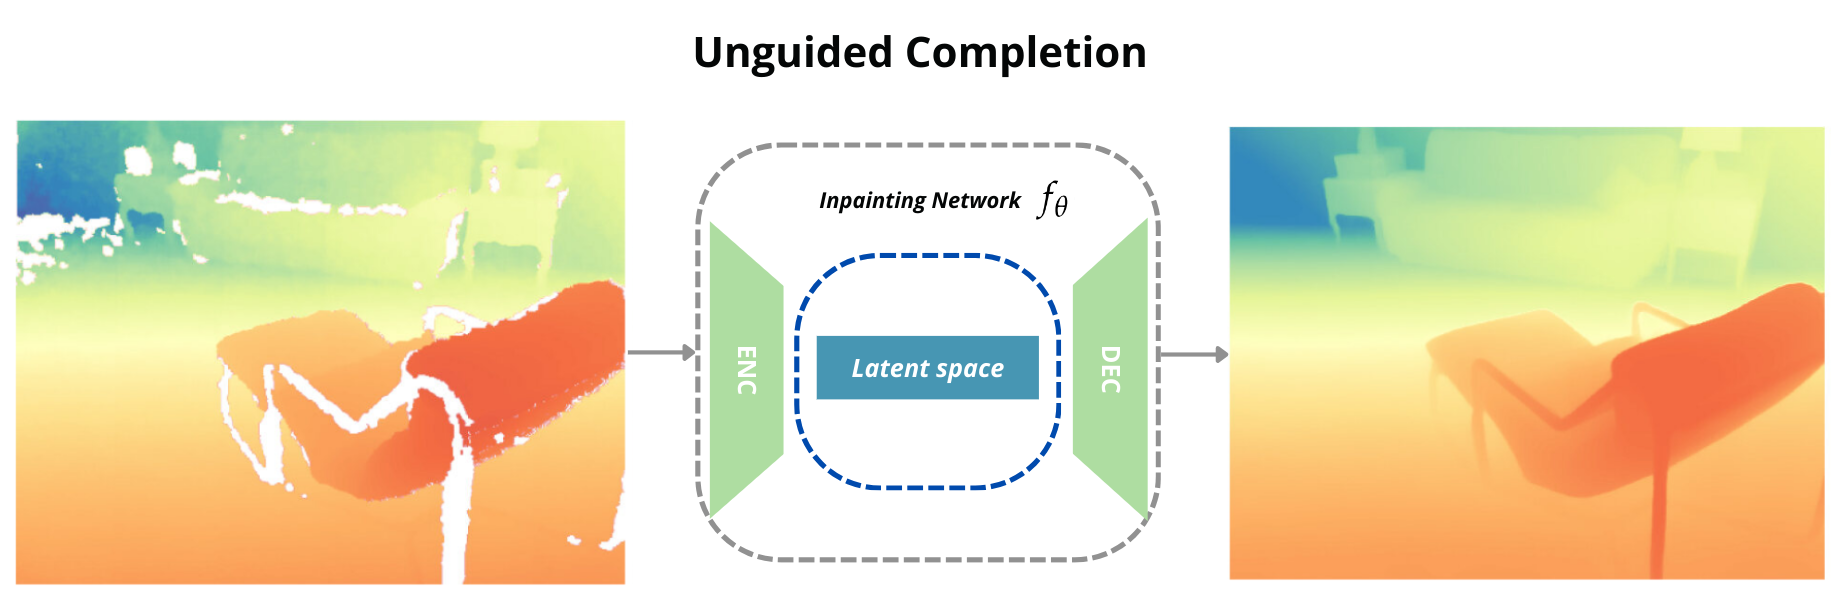
\includegraphics[width=\textwidth]{fig/unguided.png}
    \caption{Esquema de correção não-guiada.}
    \label{ung}
\end{figure}

A escolha da categoria de correção depende da quantidade de erros nas imagens. Quando há uma pequena quantidade de pixels inválidos, a correção não-guiada pode ser adequada, visto que não é necessário uma profunda extração de características dos dados. No entanto, no caso contrário, o uso de métodos guiados é indicado dado que existam grandes regiões com ausência de informação de profundidade ou que o mapa apresente uma grande esparsidade. Sendo necessário recorrer a extração dos atributos presentes na imagem RGB como bordas, contornos, estruturas de objetos não identificados pelo sensor e característica de descontinuidade de superfícies \cite{hu2022deep}.

Ainda no trabalho de \cite{hu2022deep}, nomeia-se outras subcategorias de técnicas de correção guiada. Uma delas é chamada de \textit{Early Fusion} (Figura \ref{early}) e consiste em utilizar a imagem RGB concatenada ao mapa de profundidade com erros como entrada da rede neural. Essa técnica possui a vantagem de ser simples e de baixa complexidade. A outra, conhecida como \textit{Late Fusion} (Figura \ref{late}) envolve transferir a fusão da imagem RGB com o mapa em ramos distintos da rede neural, chamados \textit{RGB Encoder-Decoder} e \textit{Depth Encoder-Decoder}.

\begin{figure}[h]
    \centering
    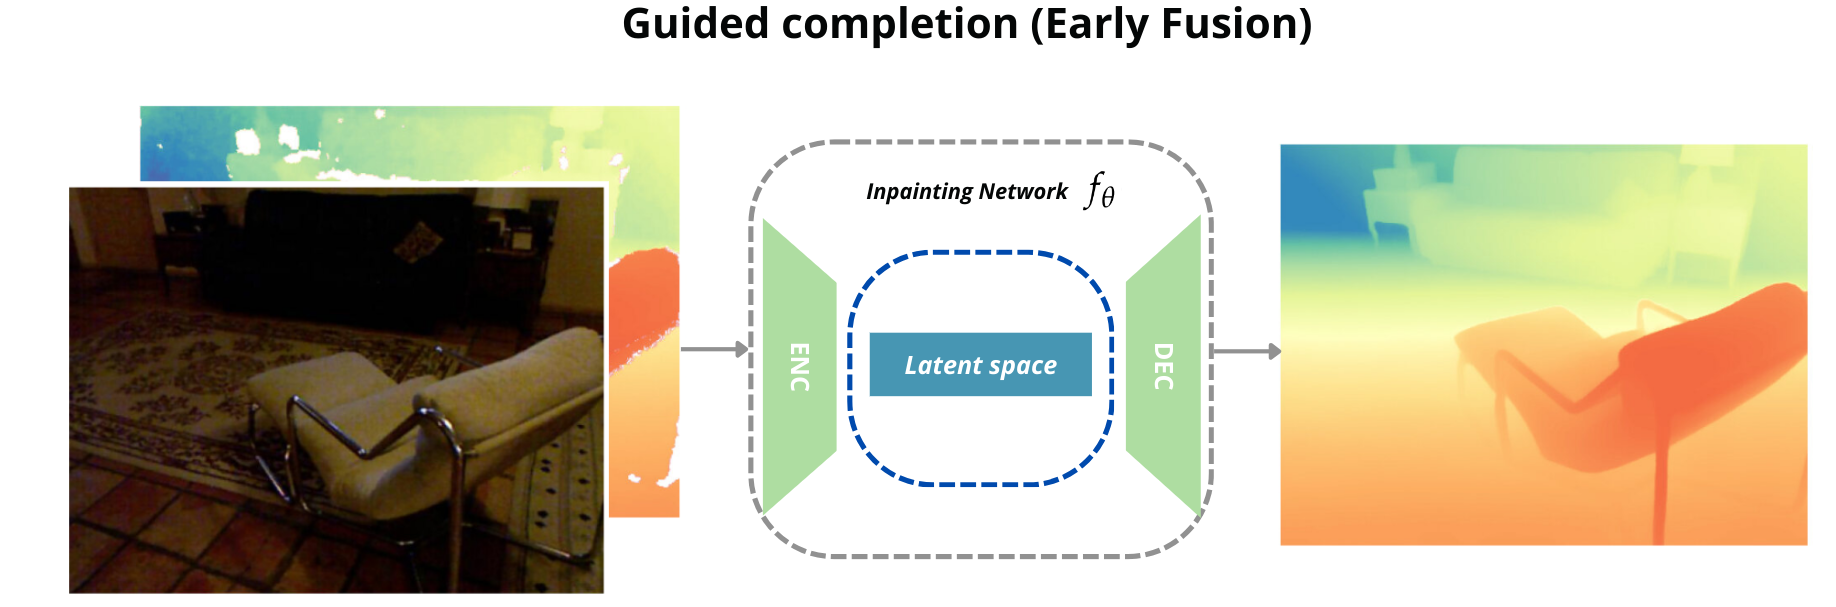
\includegraphics[width=\textwidth]{fig/earlyfusion.png}
    \caption{Esquema de correção guiada com \textit{Early Fusion}.}
    \label{early}
\end{figure}

\begin{figure}[h]
    \centering
    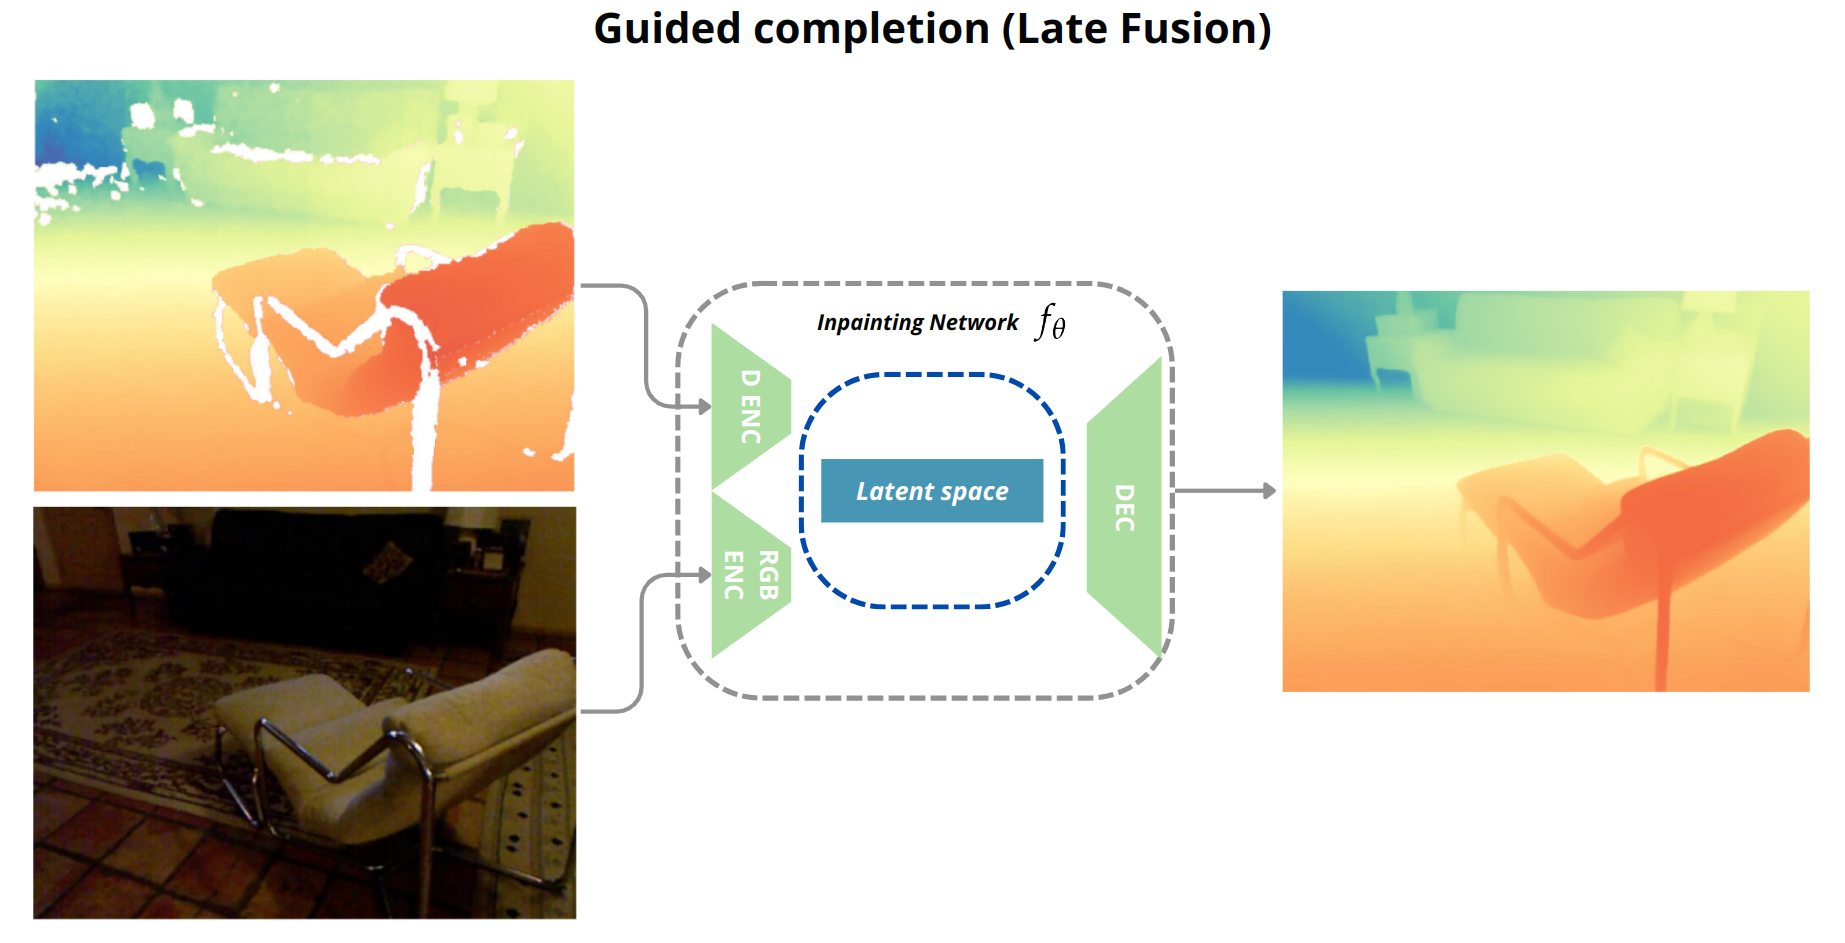
\includegraphics[width=\textwidth]{fig/latefusion.png}
    \caption{Esquema de correção guiada com \textit{Late Fusion}.}
    \label{late}
\end{figure}


\subsection{Large Mask Inpainting}

%Image inpainting is the process of completing or recovering the missing region in the image or removing some objects added to it. 

\textit{Image Inpainting} refere-se ao processo de recuperar regiões faltantes de uma imagem a partir de informação já existente \cite{elharrouss2020image}. Para sintetizar as partes indicadas, é necessário que haja o aprendizado da estrutura global da imagem, sendo imprescindível um vasto campo receptivo na rede neural. Dessa forma, é proposto por \cite{suvorov2022resolution} o sistema LaMa, \textit{Large Mask Inpainting} (Figura \ref{lama}), que é composto por elementos capazes de explorar o campo receptivo apropriado para essa tarefa, sendo eles: i) convoluções rápidas de Fourier (do inglês, \textit{Fast Fourier Convolutions}), ii) o uso de perda perceptual baseada em uma rede de segmentação e iii) uma estratégia de geração de máscaras para treinamento de alta cobertura.

\begin{figure}[h]
    \centering
    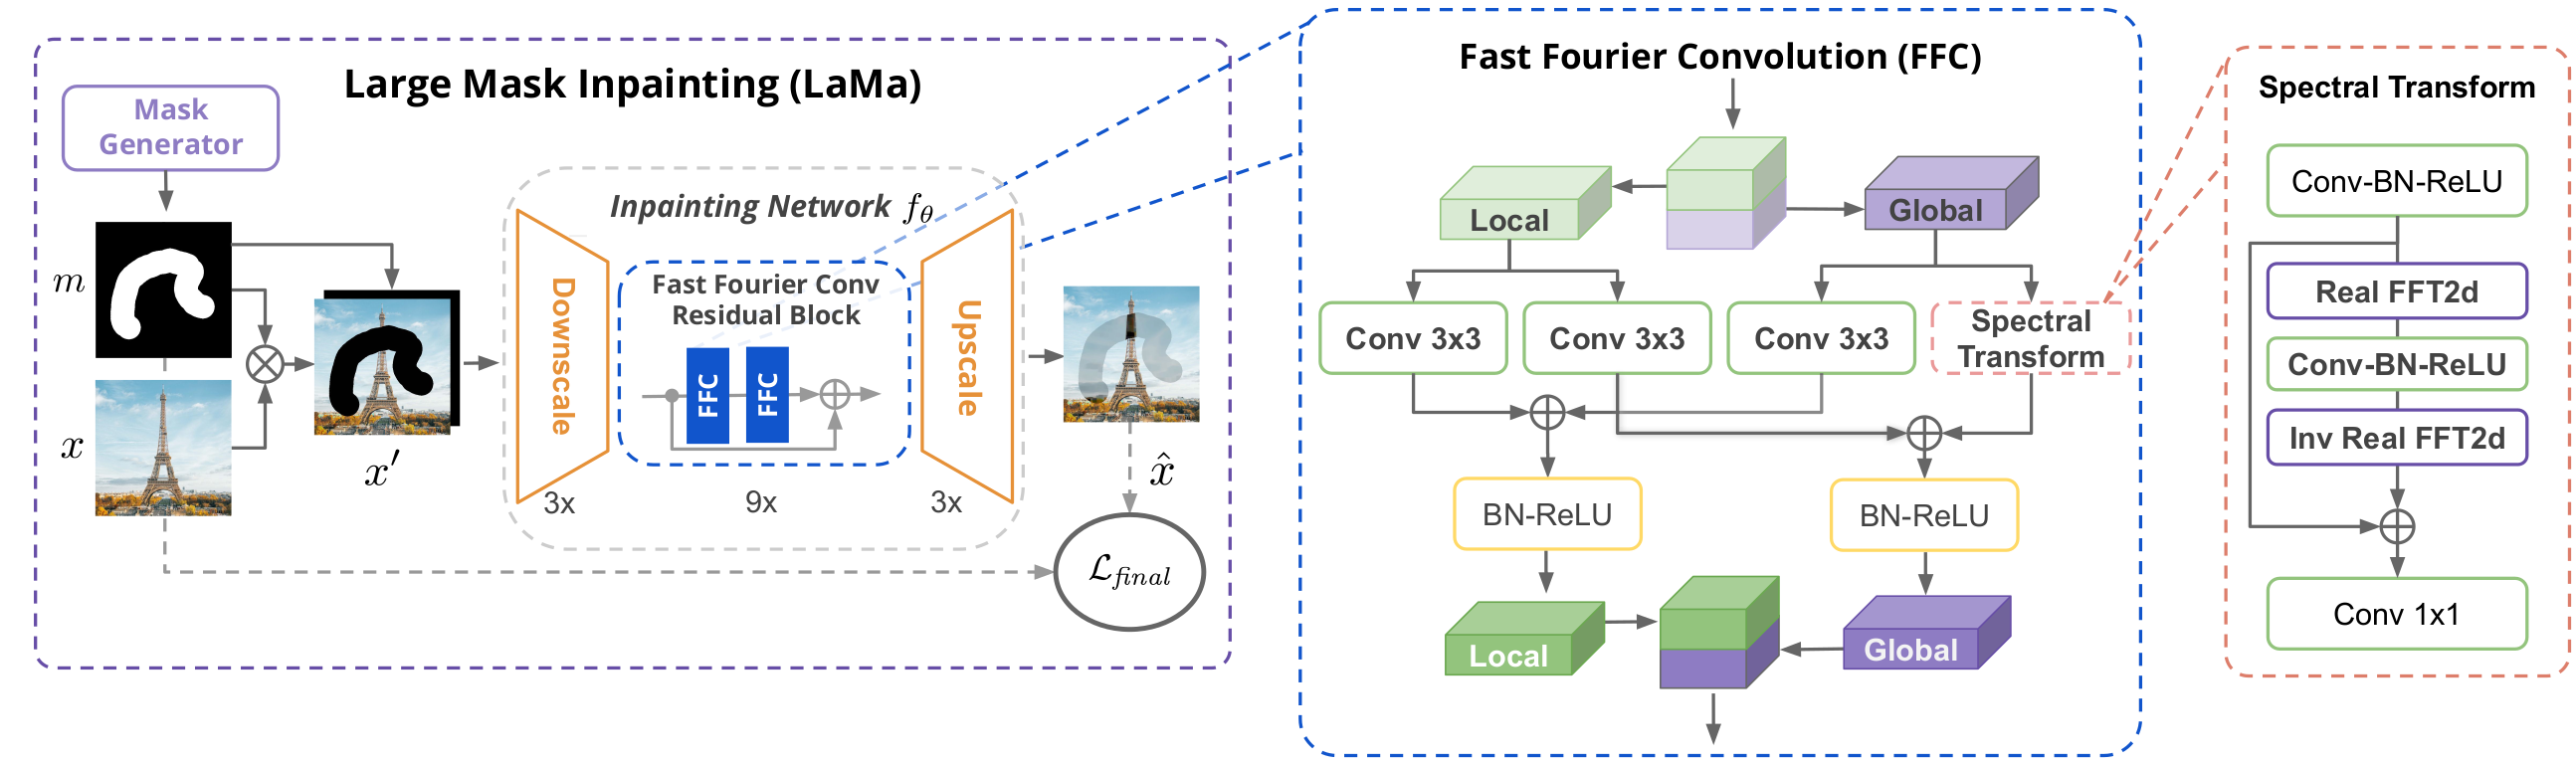
\includegraphics[width=\textwidth]{fig/lama.png}
    \caption{Esquema do método LaMa \cite{suvorov2022resolution}.}
    \label{lama}
\end{figure}

%explain receptive field?

\section{Datasets}

O presente trabalho exige um tipo de base de dados pouco encontrado na literatura, trios de imagem RGB, mapa de profundidade com erros e um outro mapa de profundidade denso e completo. De acordo com \cite{zhang2018deep}, uma das maneiras de se obter esses dados seria capturar imagens com uma câmera RGB-D de baixo custo e alinha-las com outra captura simultânea de um sensor mais preciso, porém essa abordagem é muito custosa, além de que não há disponibilidade de grandes conjuntos para treinamento.

O presente projeto pretende utilizar como base de dados principal o \textbf{Hypersim}. Um \textit{dataset} para compreensão de cenas baseado em cenas sintéticas fotorrealistas. Contendo 77.400 imagens de 461 cenas \textit{indoor} com pares de RGB e mapas de profundidade calculado deterministicamente, além de outras informações como normais de superfície, rótulos de segmentação e detecção de objetos e entre outros \cite{roberts2021hypersim}.

\section{Metodologia da Pesquisa}






    
\chapter{Resultados Preliminares}




% --- -----------------------------------------------------------------
% --- Referencias Bibliograficas. (Obrigatorio)
% --- -----------------------------------------------------------------
    \cleardoublepage
%    \bibliographystyle{acm-2} % abbrv - abnt-num
	%\bibliographystyle{plainnat}
    \bibliography{bibliografia} % arquivo fonte com a bibilografia

% --- -----------------------------------------------------------------
% --- Apendice.(Opcional)
% --- -----------------------------------------------------------------
    \cleardoublepage
    \appendix
    \begin{landscape}
        \chapter{Apêndice A}
\label{appendixA}

...
        % \include{appendixB}
        % \include{appendixC}
        % \include{appendixD}
        % \include{appendixE}
        % \include{appendixF}
        % \include{appendixG}
        % \include{appendixH}
        % \include{appendixI}
        % \include{appendixJ}
        % \include{appendixK}
        %\include{appendixL}
    \end{landscape}
\end{document}